\documentclass[11pt]{standalone}


\usepackage{amssymb} 
\usepackage{amsmath} 

\usepackage[no-math]{fontspec}
\usepackage{unicode-math}
\setmainfont{TeX Gyre Heros}
\setmathfont{Stix Two Math}

\usepackage{xcolor}

\usepackage{tikz}
\usetikzlibrary{arrows.meta, backgrounds}

\definecolor{myblue}{HTML}{CCDEE9}
\definecolor{bgcolor}{HTML}{F3F4F4}


\begin{document}
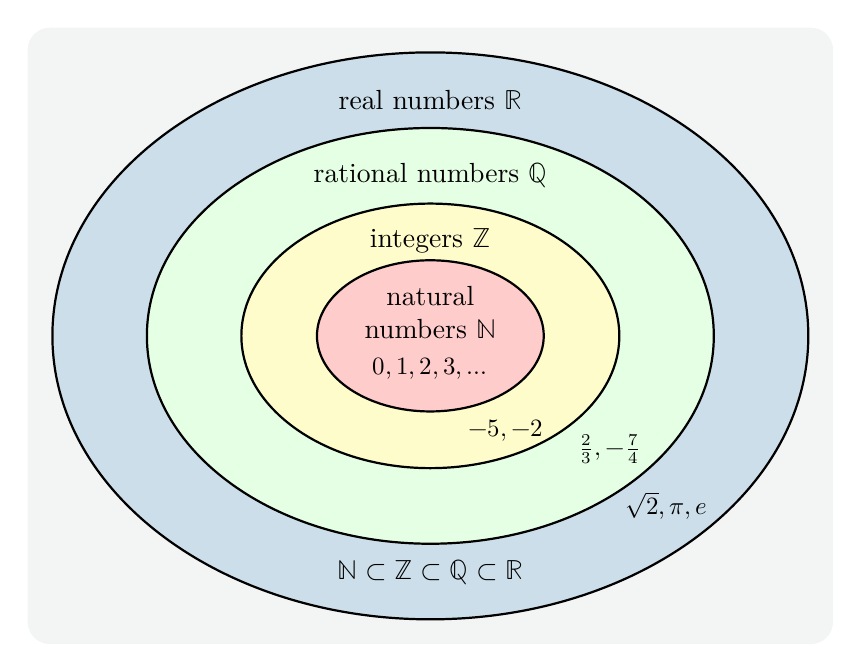
\begin{tikzpicture}[scale=1.2,
    show background rectangle,
    background rectangle/.style={fill=bgcolor, rounded corners=8pt},
    inner frame sep=0.3cm
]
  % Real numbers (outermost)
  \draw[thick, fill=myblue] (0,0) ellipse (4cm and 3cm);
  \node at (0,2.5) {real numbers $\mathbb{R}$};
  
  % Rational numbers
  \draw[thick, fill=green!10] (0,0) ellipse (3cm and 2.2cm);
  \node at (0,1.7) {rational numbers $\mathbb{Q}$};
  
  % Integers
  \draw[thick, fill=yellow!20] (0,0) ellipse (2cm and 1.4cm);
  \node at (0,1.0) {integers $\mathbb{Z}$};
  
  % Natural numbers (innermost)
  \draw[thick, fill=red!20] (0,0) ellipse (1.2cm and 0.8cm);
  \node[align=center] at (0,0.25) {natural \\numbers $\mathbb{N}$};
  
  % Example elements in each set
  \node at (0,-0.35) {\small $0, 1, 2, 3, \ldots$};
  \node at (0.8,-1.0) {\small $-5, -2$};
  \node at (1.9,-1.2) {\small $\frac{2}{3}, -\frac{7}{4}$};
  \node at (2.5,-1.8) {\small $\sqrt{2}, \pi, e$};
  
  % Subset symbols (optional)
  \node at (0,-2.5) {$\mathbb{N} \subset \mathbb{Z} \subset \mathbb{Q} \subset \mathbb{R}$};
  
\end{tikzpicture}\end{document}